\documentclass[11pt, a4paper, twoside, article, openany]{memoir}

\usepackage[utf8]{inputenc}		% Dansk input encoding (tegn)
\usepackage[english, danish]{babel}		% Danske formuleringer / orddeling
\usepackage[T1]{fontenc}		% Output-indkodning af tegnsaet (T1)

%%% Memoir indstillinger
%% Afstand mellem afsnit og videre
%% NIX PILLE - medmindre strengt nødvendigt
\setaftersubsubsecskip{6pt}	
\setbeforesubsubsecskip{ 6pt}
%\setaftersubsecskip{6pt}
%\setbeforesubsecskip{-\baselineskip}
%\setaftersecskip{6pt}
%\setbeforesecskip{-\baselineskip}
%\setaftersecskip{1ex}

\raggedbottom


%\counterwithout{section}{chapter}
\chapterstyle{section}

% ¤¤ Marginer ¤¤ %
\setlrmarginsandblock{3.5cm}{2.5cm}{*}		% \setlrmarginsandblock{Indbinding}{Kant}{Ratio}
\setulmarginsandblock{3.0cm}{2.5cm}{*}		% \setulmarginsandblock{Top}{Bund}{Ratio}
\checkandfixthelayout

%%% Font valg %%%
\usepackage{mathpazo}	%Palatinofont - matematikformler
\usepackage{eulervm}		%Palatinofont

%%% FIGURER OG TABELLER %%%
\usepackage{graphicx} 						% Haandtering af eksterne billeder (JPG, PNG, PDF)

\usepackage[export]{adjustbox}

\usepackage{subfig}

\usepackage{multirow}                		% Fletning af raekker og kolonner (\multicolumn og \multirow)
\usepackage{colortbl} 						% Farver i tabeller (fx \columncolor, \rowcolor og \cellcolor)
\usepackage[dvipsnames]{xcolor}				% Definer farver med \definecolor. Se mere: http://en.wikibooks.org/wiki/LaTeX/Colors
%\usepackage{flafter}						% Soerger for at floats ikke optraeder i teksten foer deres erence
\usepackage{float}							% Muliggoer eksakt placering af floats, f.eks. \begin{figure}[H]
\usepackage{multicol}         	        	% Muliggoer tekst i spalter
%\usepackage{rotating}						% Rotation af tekst med \begin{sideways}...\end{sideways}
\usepackage{booktabs}
\usepackage{bigstrut}	% Excel2latex måskeh
\usepackage{tabularx}

%%% ¤¤ Matematik mm. %%%
\usepackage{amsmath,amssymb,stmaryrd} 		% Avancerede matematik-udvidelser
\usepackage{mathtools}						% Andre matematik- og tegnudvidelser
\usepackage{textcomp}                 		% Symbol-udvidelser (f.eks. promille-tegn med \textperthousand )
\usepackage{siunitx}						% Flot og konsistent praesentation af tal og enheder med \si{enhed} og \SI{tal}{enhed}
\sisetup{output-decimal-marker = {,}}		% Opsaetning af \SI (DE for komma som decimalseparator) 
\sisetup{exponent-product=\cdot, output-product=\cdot}	%Eksponent er gange tegn, output produkt er gange tegn
\sisetup{digitsep = none}					%Almindeligt komma - ingen mellemrum aka. til eurokomma

%%% MISC %%%
\usepackage{listings}						% Placer kildekode i dokumentet med \begin{lstlisting}...\end{lstlisting}
\definecolor{bg}{HTML}{F0F0F0}
\lstset{language=C++,
				showstringspaces = false,
				backgroundcolor = \color{bg},
                basicstyle=\ttfamily,
                keywordstyle=\color{blue}\ttfamily,
                stringstyle=\color{red}\ttfamily,
                commentstyle=\color{green}\ttfamily,
                morecomment=[l][\color{magenta}]{\#},
                extendedchars=true,
                numbers=left, numberstyle=\tiny,		% Linjenumre
                columns=flexible,						% Kolonnejustering
                breaklines, breakatwhitespace=true,		% Bryd lange linjer
                literate=%
                {æ}{{\ae}}1
                {å}{{\aa}}1
                {ø}{{\o}}1
                {Æ}{{\AE}}1
                {Å}{{\AA}}1
                {Ø}{{\O}}1
}

\usepackage{lipsum}							% Dummy text \lipsum[..]
\usepackage[shortlabels]{enumitem}			% Muliggoer enkelt konfiguration af lister
\usepackage{pdfpages}						% Goer det muligt at inkludere pdf-dokumenter med kommandoen \includepdf[pages={x-y}]{fil.pdf}	
\pdfoptionpdfminorversion=6					% Muliggoer inkludering af pdf dokumenter, af version 1.6 og hoejere

%	¤¤ Afsnitsformatering ¤¤ %
%\setlength{\parindent}{0mm}           		% Stoerrelse af indryk
\setlength{\parskip}{1.5mm}          		% Afstand mellem afsnit ved brug af double Enter
\linespread{1,1}							% Linie afstand

\usepackage{tikz}

% ¤¤ Visuelle  ¤¤ %
\usepackage[colorlinks]{hyperref}			% Danner klikbare referencer (hyperlinks) i dokumentet.
\hypersetup{colorlinks = true,				% Opsaetning af farvede hyperlinks (interne links, citeringer og URL)
	linkcolor = black,
	citecolor = black,
	urlcolor = black
}
\usepackage{url}

%%% REFERENCER %%%
%\usepackage{xr}
%\externaldocument{../dokumentation/dokumentation.tex}

%%% Referencer / Bibliografi %%%
\usepackage[backend=bibtex, sorting=none, style=numeric]{biblatex}
\bibliography{bibliography.bib}

\usepackage[draft, danish]{fixme}
\fxsetup{layout=footnote}

\graphicspath{{../fig/}{../fig}{fig/}{./}}

\usepackage{titlesec}

\setcounter{secnumdepth}{3}

\titleformat{\paragraph}
{\normalfont\normalsize\bfseries}{\theparagraph}{1em}{}
\titlespacing*{\paragraph}
{0pt}{3.25ex plus 1ex minus .2ex}{1.5ex plus .2ex}


%%%% Opsætning af dokument %%%%
\newcommand{\forfatter}{Gruppe xx}
\newcommand{\fag}{yy}
\newcommand{\titel}{zz}
\date{}

\author{\forfatter}
\title{\titel}


\setlength{\beforechapskip}{10pt}
\setlength{\afterchapskip}{10pt}

\begin{document}

\selectlanguage{english}
	
\chapter{Requirements specification}

The requirements for the product are prioritized using the MoSCoW method. Using this, the requirements for the product are divided into four sections, where the most important elements are given the highest priority. \textbf{Must} are the requirements that are an absolute necessity for the product. \textbf{Should} are the requirements that are also of high priority, but not quite mandatory. \textbf{Could} are requirements which may be met, if the time and other constraints of the project allow for it. \textbf{Won't} are the requirements the product will not meet, but could be developed at a later point in its lifetime.  

\noindent The following priorities have been chosen for this project:
\begin{itemize}
	\item[\textbf{Must}]
	\begin{itemize}
		\item Navigate waypoints from user input
		\item Be compatible with NMEA protocol GPS input
		\item Use GPS for localization
		\item Implement a PID control loop
	\end{itemize}
	\item[\textbf{Should}]
	\begin{itemize}
		\item Control thrusters in two-thruster catamaran
		\item Use a graphical user interface for user interaction
		\item Be able to change the PID parameters
	\end{itemize}
	\item[\textbf{Could}] 
	\begin{itemize}
		\item Control wheel in outboard motor on boat
		\item Be generic enough to use with other engine types
	\end{itemize}
	\item[\textbf{Won't}]
	\begin{itemize}
		\item Use pylogon-coverage for a specified area
		\item Avoid obstacles
	\end{itemize}
\end{itemize}

Figure \ref{fig:rich_image} below shows an illustration of the usage scenario for the Boat autopilot system. A technician or a user accesses the system using an interface. This interface communicates with the system using wireless communication, and the system performs the appropriate actions, for example following a curved path to cover a specified area. 

\begin{figure}[H]
	\centering
	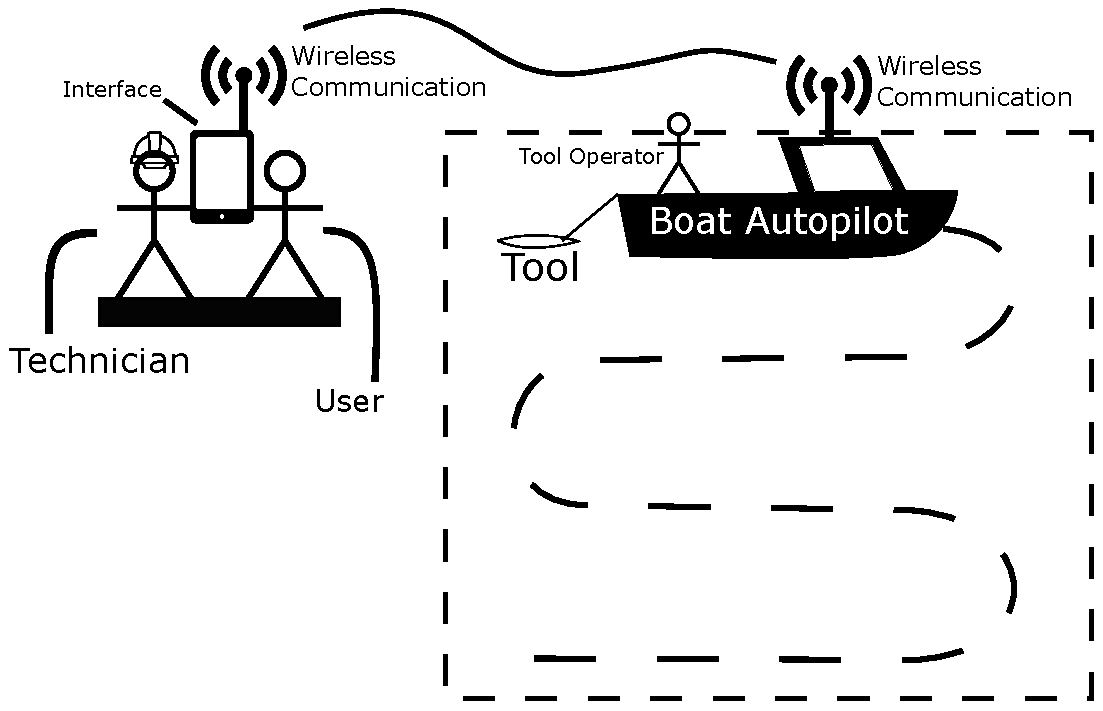
\includegraphics[width=1\linewidth]{Images/Introduction/rich_image}
	\caption{Rich image}
	\label{fig:rich_image}
\end{figure}

Figure \ref{fig:general_sd} shows a general, and simplified, sequence of events for the system.

\begin{figure}[H]
	\centering
	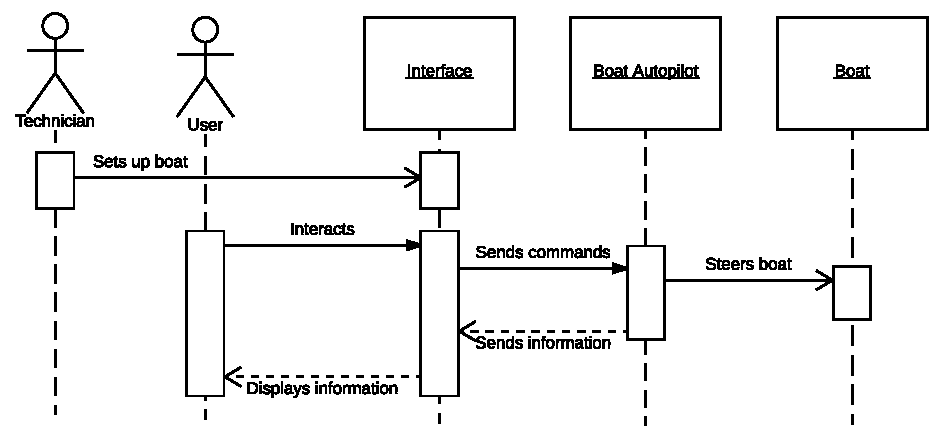
\includegraphics[width=1\linewidth]{Images/Introduction/General_SD}
	\caption{General sequence diagram}
	\label{fig:general_sd}
\end{figure}

At this point it seemed appropriate to consider the design of the user interface because it describes how the actors interact with the system, which makes it possible to specify the Use cases of the system. 

\begin{figure}[H]
	\centering
	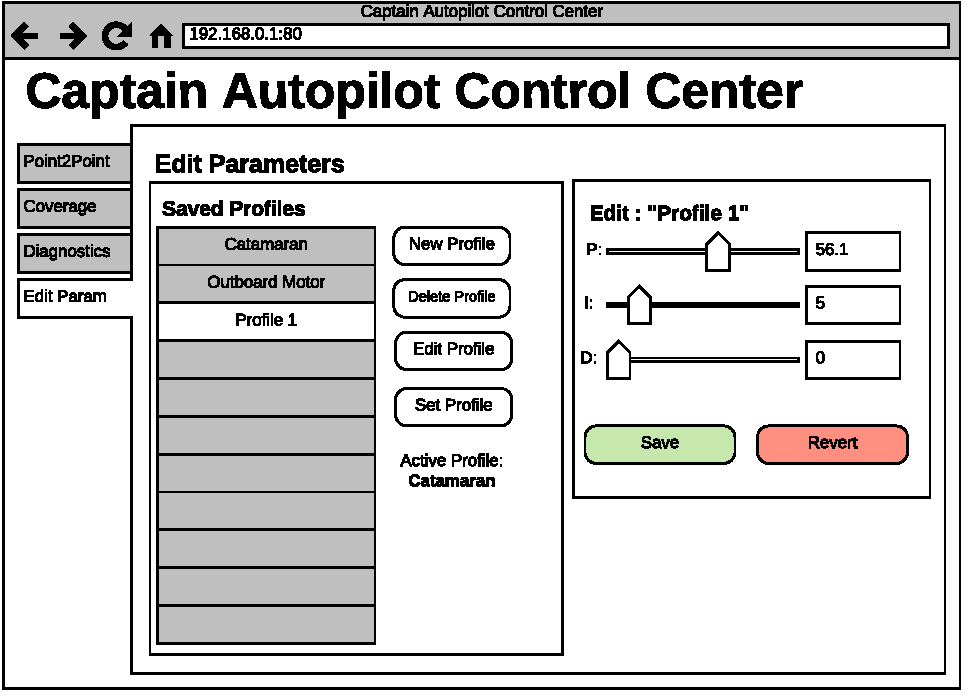
\includegraphics[width=1\linewidth]{Images/Requirements_specification/UI_Mockup_Edit_param.pdf}
	\caption{Mockup for Edit parameter menu}
	\label{fig:mockupparam}
\end{figure}

Figure \ref{fig:mockupparam} shows the Edit Param menu of the user interface. As seen in the UI, the technician can create and edit new profiles for the Controller, and set which one is actively running in the control loop. 

\begin{figure}[H]
	\centering
	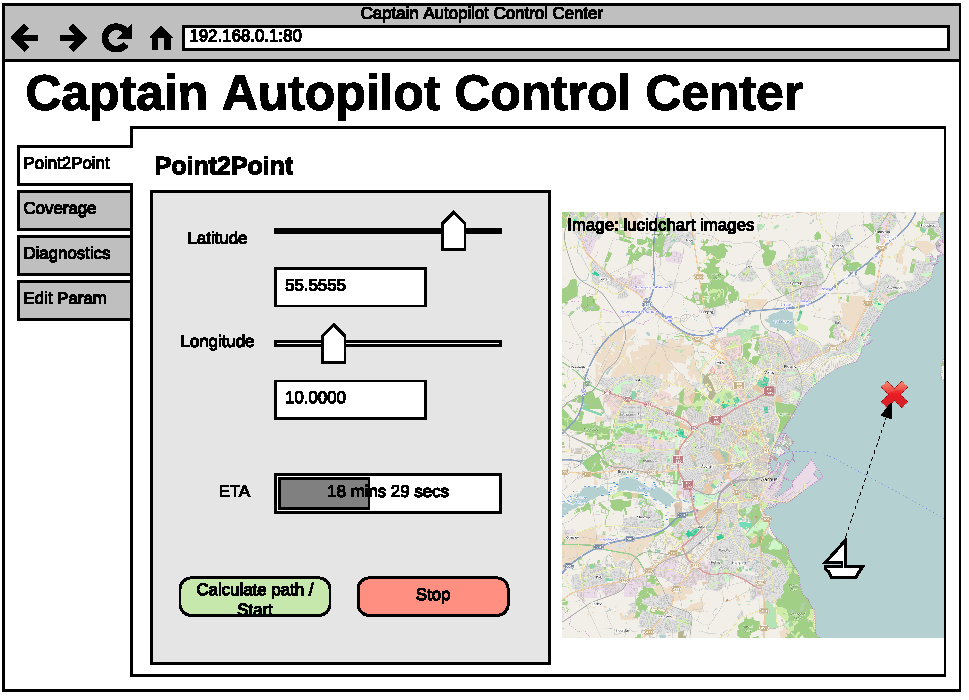
\includegraphics[width=1\linewidth]{Images/Requirements_specification/UI_Mockup_Point_to_point.pdf}
	\caption{Mockup for Point to point menu}
	\label{fig:mockupp2p}
\end{figure}

Figure \ref{fig:mockupp2p} shows the Point to point menu of the user interface. In this menu, the user can specify a destination either on a map or by inputting coordinates, then ask the system to calculate a path there, and finally to proceed to the destination. If needed, the user can also stop the boat.

\begin{figure}[H]
	\centering
	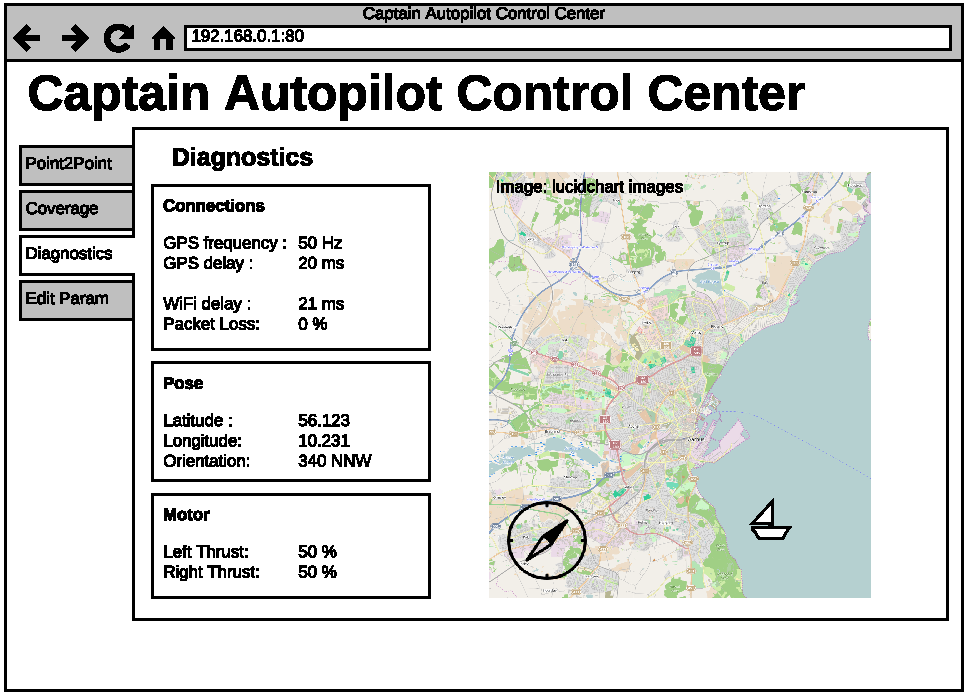
\includegraphics[width=1\linewidth]{Images/Requirements_specification/UI_Mockup_Diagnostics.pdf}
	\caption{Mockup for Diagnostics menu}
	\label{fig:mockupdiag}
\end{figure}

Figure \ref{fig:mockupdiag} shows the Diagnostics menu of the user interface. Here, the system status is shown to make troubleshooting easier.

\begin{figure}[H]
	\centering
	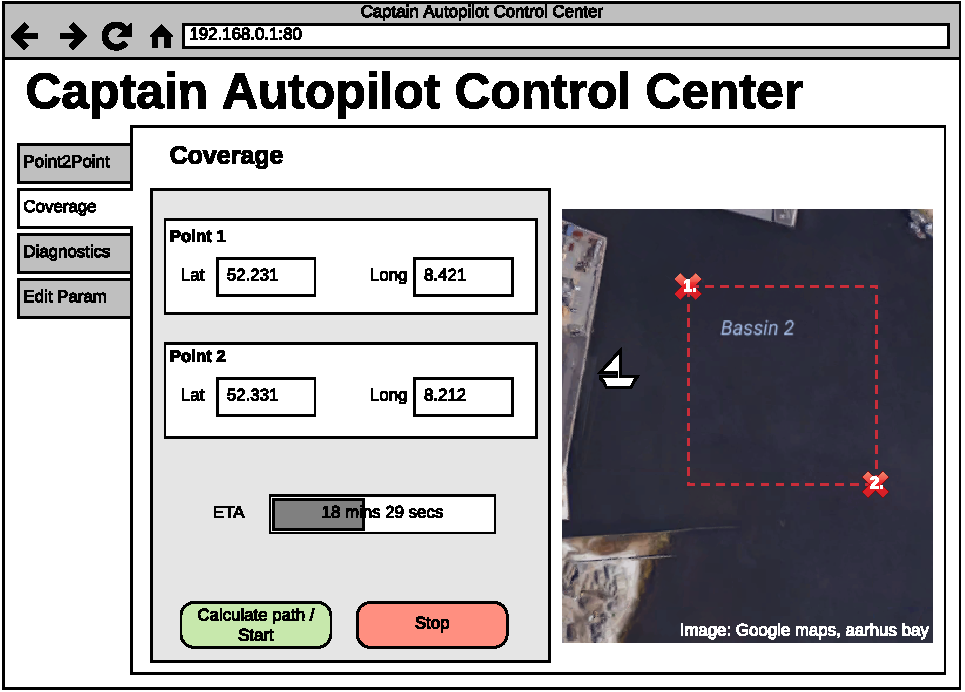
\includegraphics[width=1\linewidth]{Images/Requirements_specification/UI_Mockup_Coverage.pdf}
	\caption{Mockup for Coverage menu}
	\label{fig:mockupcover}
\end{figure}

Figure \ref{fig:mockupcover} shows the Coverage menu of the user interface. Here, the user can specify two opposing edges of a rectangle for the system to cover. The user can then ask the system to calculate a curved path through this area, and finally to proceed. There is, like in the Point to point menu, a stop function for convenience.

\begin{figure}[H]
	\centering
	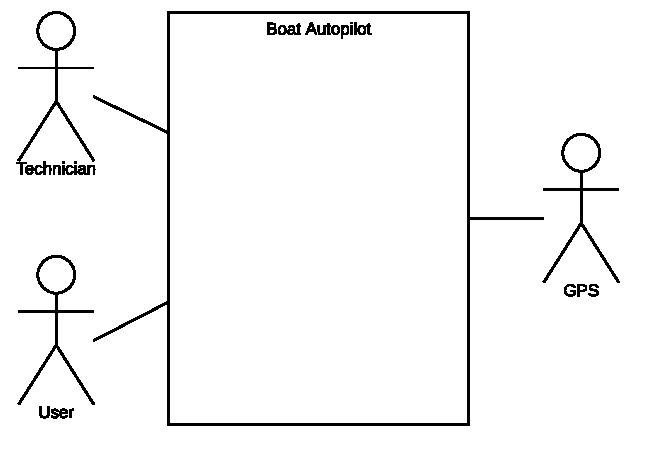
\includegraphics{Images/Requirements_specification/Actor_context_diagram}
	\caption{Actor context diagram}
	\label{fig:actorcontextdiagram}
\end{figure}

Figure \ref{fig:actorcontextdiagram} shows an actor context diagram for the system. The technician and the user are primary actors, and the GPS is a secondary actor.

\begin{figure}[H]
	\centering
	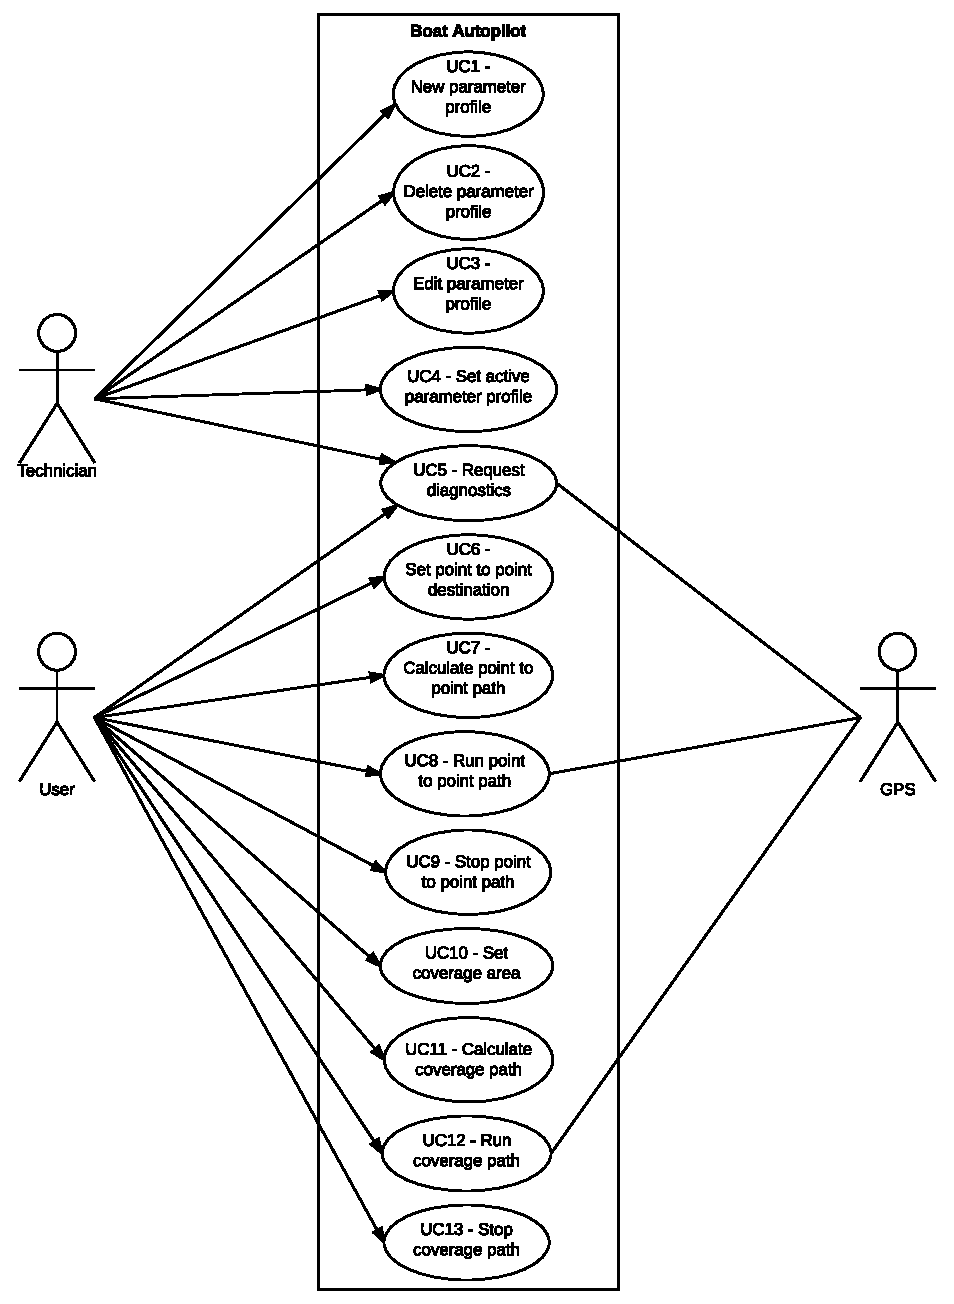
\includegraphics[width=0.9\linewidth]{Images/Requirements_specification/Usecase_diagram}
	\caption{Use case diagram}
	\label{fig:usecasediagram}
\end{figure}

Figure \ref{fig:usecasediagram} shows the use cases for the system, and the arrows show which actors are involved in each. The use cases are broadly based on the UI mockups.

\section{Actor description}
The following section describes the system's actors. Every actor has a type and a short description of its function and impact on the system.

\begin{framed}
	\subsection{Actor: Technician}
	\subsubsection*{Type:}
	Primary
	
	\subsubsection*{Description:}
	A technician with knowledge of the system.
	
\end{framed}

\begin{framed}
	\subsection{Actor: User}
	\subsubsection*{Type:}
	Primary
	
	\subsubsection*{Description:}
	The user, or customer. 
\end{framed}

\begin{framed}
	\subsection{Actor: GPS}
	\subsubsection*{Type:}
	Secondary
	
	\subsubsection*{Description:}
	The global positioning system.
	
\end{framed}

\pagebreak

\section{Fully dressed Use cases }

\begin{framed}
	\subsection{Use case 1 - New parameter profile}
	\subsubsection*{Goal:}
	To create a new parameter profile for the controller
	
	\subsubsection*{Initialization:}
	Technician
	
	\subsubsection*{Actors:}
	Technician (primary)
	
	\subsubsection*{References:}
	None
	
	\subsubsection*{Simultaneous occurrences:}
	One
	
	\subsubsection*{Prerequisite:}
	"Edit parameter" menu is opened in user interface
	
	\subsubsection*{Result:}
	A new parameter profile has been created.
	
	\subsubsection*{Main scenario:}
	\begin{enumerate}
		\item The technician selects "New Profile" button as seen on figure \ref{fig:mockupparam}.
		\item A new parameter profile is added to the list of parameter profiles, all parameters are set to default values.
		\item The selected parameter profile values are displayed on the user interface
	\end{enumerate}	
\end{framed}

\begin{framed}
	\subsection{Use case 2 - Delete parameter profile}
	\subsubsection*{Goal:}
	To delete a parameter profile for the controller
	
	\subsubsection*{Initialization:}
	Technician
	
	\subsubsection*{Actors:}
	Technician (primary)
	
	\subsubsection*{References:}
	None
	
	\subsubsection*{Simultaneous occurrences:}
	One
	
	\subsubsection*{Prerequisite:}
	\begin{itemize}
		\item "Edit parameter" menu is opened in user interface
		\item A parameter profile must exist.
	\end{itemize}
	
	\subsubsection*{Result:}
	A parameter profile has been deleted
	
	\subsubsection*{Main scenario:}
	\begin{enumerate}
		\item The technician selects a desired parameter profile to delete
		\item The technician selects "Delete Profile" button as seen on figure \ref{fig:mockupparam}.
		\item The selected profile is deleted from the list of parameter profiles. [Extension 1]
	\end{enumerate}	
	
	\subsubsection*{Extension 1: Active profile deleted}
	\begin{enumerate}
		\item If the active profile is deleted, no active profile is set.
	\end{enumerate}
	
	
\end{framed}

\begin{framed}
	\subsection{Use case 3 - Edit parameter profile}
	\subsubsection*{Goal:}
	To edit an existing parameter profile 
	
	\subsubsection*{Initialization:}
	Technician
	
	\subsubsection*{Actors:}
	Technician (primary)
	
	\subsubsection*{References:}
	None
	
	\subsubsection*{Simultaneous occurrences:}
	One
	
	\subsubsection*{Prerequisite:}
	\begin{itemize}
		\item "Edit parameter" menu is opened in user interface
		\item A parameter profile must exist.
	\end{itemize}
	
	
	\subsubsection*{Result:}
	The parameter profile has been edited
	
	\subsubsection*{Main scenario:}
	\begin{enumerate}
		\item The technician selects a desired parameter profile to edit
		\item Then the technician selects "Edit Profile" as seen on figure \ref{fig:mockupparam}
		\item The selected parameter profile values are displayed on the user interface
		\item The technician edits the parameter values of the profile
		\item The technician selects "Save" [Extension 1]
		\item The old parameter profile is overwritten with the new values.
	\end{enumerate}	
	
	\subsubsection*{Extension 1: Revert}
	\begin{enumerate}
		\item The technician selects "Revert"
		\item The old parameter profile is not overwritten. The old values are kept
		\item The user interface displays the old values
	\end{enumerate}
\end{framed}

\begin{framed}
	\subsection{Use case 4 - Set active parameter profile}
	\subsubsection*{Goal:}
	To set a parameter profile as active.
	
	\subsubsection*{Initialization:}
	Technician
	
	\subsubsection*{Actors:}
	Technician (primary)
	
	\subsubsection*{References:}
	None
	
	\subsubsection*{Simultaneous occurrences:}
	One
	
	\subsubsection*{Prerequisite:}
	\begin{itemize}
		\item "Edit parameter" menu is opened in user interface
		\item A parameter profile must exist.
	\end{itemize}
	
	\subsubsection*{Result:}
	The parameter profile has been set as active
	
	\subsubsection*{Main scenario:}
	\begin{enumerate}
		\item The technician selects a desired parameter profile to activate
		\item The technician then selects "Set Profile" as seen on figure \ref{fig:mockupparam}
		\item The selected parameter profile has been set as active.
		\item The name of the active profile is displayed on the user interface.
		\item The boat parameters are updated with the newly activated parameter profile values.
	\end{enumerate}
\end{framed}

\begin{framed}
	\subsection{Use case 5 - Request diagnostics}
	\subsubsection*{Goal:}
	To display all diagnostics data
	
	\subsubsection*{Initialization:}
	Technician or user
	
	\subsubsection*{Actors:}
	\begin{itemize}
		\item Technician (primary)
		\item User (primary)
		\item GPS (secondary)
	\end{itemize}
	
	\subsubsection*{References:}
	None
	
	\subsubsection*{Simultaneous occurrences:}
	One
	
	\subsubsection*{Prerequisite:}
	None
	
	\subsubsection*{Result:}
	All diagnostics data are displayed on the user interface
	
	\subsubsection*{Main scenario:}
	\begin{enumerate}
		\item The primary actor selects the "Diagnostics" menu in the user interface as seen on figure \ref{fig:mockupdiag}.
		\item The diagnostics data is displayed on the user interface. 
	\end{enumerate}
\end{framed}



\begin{framed}
	\subsection{Use case 6 - Set point to point destination}
	\subsubsection*{Goal:}
	To set a point to point destination
	
	\subsubsection*{Initialization:}
	User
	
	\subsubsection*{Actors:}
	User (primary)
	
	\subsubsection*{References:}
	None
	
	\subsubsection*{Simultaneous occurrences:}
	One
	
	\subsubsection*{Prerequisite:}
	\begin{itemize}
		\item The user interface has an updated map
		\item The "Point to point" menu is opened in user interface
	\end{itemize}
	
	\subsubsection*{Result:}
	A destination has been defined.
	
	\subsubsection*{Main scenario:}
	\begin{enumerate}
		\item The user selects a desired position on the map as seen on figure \ref{fig:mockupp2p}.
		\item \label{uc4.2} The user interface displays the selected position on the map
		\item The user interface displays the selected position as coordinates
	\end{enumerate}	
	
	\subsubsection*{Alternate flow 1: Coordinate input} 
	\begin{enumerate}
		\item The user inputs latitude and longitude in the user interface
		\item The main scenario is continued from \ref{uc4.2}
	\end{enumerate}
\end{framed}	

\begin{framed}
	\subsection{Use case 7 - Calculate point to point path}
	\subsubsection*{Goal:}
	A path to the destination has been calculated.
	
	\subsubsection*{Initialization:}
	User
	
	\subsubsection*{Actors:}
	User (primary)
	
	\subsubsection*{References:}
	None
	
	\subsubsection*{Simultaneous occurrences:}
	One 
	
	\subsubsection*{Prerequisite:}
	\begin{itemize}
		\item Use case 6 - Set point to point destination has been completed
		\item The user interface has an updated map
		\item The "Point to point" menu is opened in user interface
		\item The boat must not be running a navigation task.
	\end{itemize}
	
	\subsubsection*{Result:}
	A path to the destination has been calculated.
	
	\subsubsection*{Main scenario:}
	\begin{enumerate}
		\item The user selects "Calculate path" from the user interface as seen on figure \ref{fig:mockupp2p}.
		\item A path is calculated and displayed on the map. 
		\item The "Calculate path" option is changed to "Start"
	\end{enumerate}	
\end{framed}	


\begin{framed}
	\subsection{Use case 8 - Run point to point path}
	\subsubsection*{Goal:}
	The boat reaches the point to point destination
	
	\subsubsection*{Initialization:}
	User
	
	\subsubsection*{Actors:}
	User (primary)
	
	\subsubsection*{References:}
	Use case 7 - Calculate point to point path
	
	\subsubsection*{Simultaneous occurrences:}
	One 
	
	\subsubsection*{Prerequisite:}
	\begin{itemize}
		\item The user interface has an updated map
		\item The "Point to point" menu is opened in user interface
		\item Use case 7 - Calculate point to point path has been completed
		\item There must be an active parameter profile.
		\item The boat must not be running a navigation task.
	\end{itemize}
	
	\subsubsection*{Result:}
	The destination is reached
	
	\subsubsection*{Main scenario:}
	\begin{enumerate}
		\item The user selects "Start" as seen on figure \ref{fig:mockupp2p}.
		\item The "Start" button on the user interface changes to read "Running...".
		\item The boat runs a control loop based on direction data from the calculated path.
		\item The position of the boat on the user interface map is continually updated using GPS.
		\item The ETA is continually calculated and displayed on the user interface.
		\item When the boat reaches its destination it stops.
		\item On the user interface the "Running..." button is replaced by the "Calculate path" button.
	\end{enumerate}	
\end{framed}	

\begin{framed}
	\subsection{Use case 9 - Stop point to point path}
	\subsubsection*{Goal:}
	The boat stops while running point to point navigation
	
	\subsubsection*{Initialization:}
	User
	
	\subsubsection*{Actors:}
	User (primary)
	
	\subsubsection*{References:}
	Use case 8 - Run point to point path
	
	\subsubsection*{Simultaneous occurrences:}
	One 
	
	\subsubsection*{Prerequisite:}
	\begin{itemize}
		\item The user interface has an updated map
		\item The "Point to point" menu is opened in user interface
		\item Use case 8 - Run point to point is running
		\item There must be an active parameter profile.
		
	\end{itemize}
	
	\subsubsection*{Result:}
	The boat has stopped
	
	\subsubsection*{Main scenario:}
	\begin{enumerate}
		\item The user selects "Stop" as seen on figure \ref{fig:mockupp2p}.
		\item The "Running..." button changes to the "Calculate path" button.
		\item The boat turns off its motors and comes to a halt.
	\end{enumerate}	
\end{framed}	

\begin{framed}
	\subsection{Use case 10 - Set coverage area}
	\subsubsection*{Goal:}
	To specify an area to cover.
	
	\subsubsection*{Initialization:}
	User
	
	\subsubsection*{Actors:}
	User (primary)
	
	\subsubsection*{References:}
	None
	
	\subsubsection*{Simultaneous occurrences:}
	One
	
	\subsubsection*{Prerequisite:}
	\begin{itemize}
		\item The user interface has an updated map
		\item The "Coverage" menu is opened in user interface
	\end{itemize}
	
	\subsubsection*{Result:}
	A coverage area has been defined
	
	\subsubsection*{Main scenario:}
	\begin{enumerate}
		\item The user selects two positions on the map which encapsulates a rectangle. One of the points is labeled "1", this specifies the starting point of the coverage route, the other is labeled "2" indicating the endpoint as seen on figure \ref{fig:mockupcover}.
		\item \label{uc10.2} The user interface displays the selected rectangle on the map, including the staring point "1" and endpoint "2".
		\item The user interface displays the selected points as coordinates.
	\end{enumerate}	
	
	\subsubsection*{Alternate flow 1: Coordinate inputs}
	\begin{enumerate}
		\item The user inputs latitude and longitude for each point "1" and "2" in the user interface.
		\item The main scenario is continued from \ref{uc10.2}
	\end{enumerate}
\end{framed}	

\begin{framed}
	\subsection{Use case 11 - Calculate coverage path}
	\subsubsection*{Goal:}
	To calculate a path that covers an area.
	
	\subsubsection*{Initialization:}
	User
	
	\subsubsection*{Actors:}
	User (primary)
	
	\subsubsection*{References:}
	Use case 10 - Set coverage area
	
	\subsubsection*{Simultaneous occurrences:}
	One 
	
	\subsubsection*{Prerequisite:}
	\begin{itemize}
		\item The user interface has an updated map
		\item The "Coverage" menu is opened in user interface.
		\item The area to cover must be defined.
		\item The boat must not be running a navigation task.
	\end{itemize}
	
	\subsubsection*{Result:}
	A path to the destination has been calculated.
	
	\subsubsection*{Main scenario:}
	\begin{enumerate}
		\item The user selects "Calculate path" from the user interface as seen on figure \ref{fig:mockupcover}.
		\item A path is calculated and displayed on the map. 
		\item The "Calculate path" option is changed to "Start"
	\end{enumerate}	
\end{framed}	

\begin{framed}
	\subsection{Use case 12 - Run coverage path}
	\subsubsection*{Goal:}
	The boat completes its coverage path.
	
	\subsubsection*{Initialization:}
	User
	
	\subsubsection*{Actors:}
	User (primary)
	
	\subsubsection*{References:}
	Use case 11 - Calculate coverage path
	
	\subsubsection*{Simultaneous occurrences:}
	One 
	
	\subsubsection*{Prerequisite:}
	\begin{itemize}
		\item The user interface has an updated map
		\item The "Coverage" menu is opened in user interface
		\item Use case 11 - Calculate coverage path has been completed
		\item There must be an active parameter profile.
		\item The boat must not be running a navigation task.
	\end{itemize}
	
	\subsubsection*{Result:}
	The coverage path is completed.
	
	\subsubsection*{Main scenario:}
	\begin{enumerate}
		\item The user selects "Start" as seen on figure \ref{fig:mockupcover}.
		\item The "Start" button on the user interface changes to read "Running...".
		\item The boat runs a control loop based on direction data from the calculated coverage path.
		\item The position of the boat on the user interface map is continually updated using GPS.
		\item The ETA is continually calculated and displayed on the user interface.
		\item When the boat reaches its destination, it stops.
		\item On the user interface the "Running..." button is replaced by a "Calculate path" button.
	\end{enumerate}	
\end{framed}	

\begin{framed}
	\subsection{Use case 13 - Stop point to point path}
	\subsubsection*{Goal:}
	The boat stops while running coverage navigation
	
	\subsubsection*{Initialization:}
	User
	
	\subsubsection*{Actors:}
	User (primary)
	
	\subsubsection*{References:}
	Use case 12 - Run coverage path
	
	\subsubsection*{Simultaneous occurrences:}
	One 
	
	\subsubsection*{Prerequisite:}
	\begin{itemize}
		\item The user interface has an updated map
		\item The "Coverage" menu is opened in user interface
		\item Use case 12 - Run coverage path is running
		\item There must be an active parameter profile.
		
	\end{itemize}
	
	\subsubsection*{Result:}
	The boat has stopped
	
	\subsubsection*{Main scenario:}
	\begin{enumerate}
		\item The user selects the "Stop" button as seen on figure \ref{fig:mockupcover}.
		\item The "Running..." button changes to a "Calculate path" button.
		\item The boat turns off its motors and comes to a halt.
	\end{enumerate}	
\end{framed}	

\section{Non-functional requirements}
Since the physical constraints of the end-system are unknown, there are no non-functional requirements at present.

\end{document}